\documentclass[a4paper,11pt]{article}
\usepackage{amsmath,amsthm,amsfonts,amssymb,amscd,amstext,vmargin,graphics,graphicx,tabularx,multicol} 
\usepackage[francais]{babel}
\usepackage[utf8]{inputenc}  
\usepackage[T1]{fontenc} 
\usepackage{pstricks-add,tikz,tkz-tab,variations}
\usepackage[autolanguage,np]{numprint} 

\setmarginsrb{1.5cm}{0.5cm}{1cm}{0.5cm}{0cm}{0cm}{0cm}{0cm} %Gauche, haut, droite, haut
\newcounter{numexo}
\newcommand{\exo}[1]{\stepcounter{numexo}\noindent{\bf \underline{Exercice~\thenumexo}}}
\reversemarginpar


\newcounter{enumtabi}
\newcounter{enumtaba}
\newcommand{\q}{\stepcounter{enumtabi} \theenumtabi.  }
\newcommand{\qa}{\stepcounter{enumtaba} (\alph{enumtaba}) }
\newcommand{\initq}{\setcounter{enumtabi}{0}}
\newcommand{\initqa}{\setcounter{enumtaba}{0}}

\newcommand{\be}{\begin{enumerate}}
\newcommand{\ee}{\end{enumerate}}
\newcommand{\bi}{\begin{itemize}}
\newcommand{\ei}{\end{itemize}}
\newcommand{\bp}{\begin{pspicture*}}
\newcommand{\ep}{\end{pspicture*}}
\newcommand{\bt}{\begin{tabular}}
\newcommand{\et}{\end{tabular}}
\renewcommand{\tabularxcolumn}[1]{>{\centering}m{#1}} %(colonne m{} centrée, au lieu de p par défault) 
\newcommand{\tnl}{\tabularnewline}

\newcommand{\bmul}[1]{\begin{multicols}{#1}}
\newcommand{\emul}{\end{multicols}}

\newcommand{\trait}{\noindent \rule{\linewidth}{0.2mm}}
\newcommand{\hs}[1]{\hspace{#1}}
\newcommand{\vs}[1]{\vspace{#1}}

\newcommand{\N}{\mathbb{N}}
\newcommand{\Z}{\mathbb{Z}}
\newcommand{\R}{\mathbb{R}}
\newcommand{\C}{\mathbb{C}}
\newcommand{\Dcal}{\mathcal{D}}
\newcommand{\Ccal}{\mathcal{C}}
\newcommand{\mc}{\mathcal}

\newcommand{\vect}[1]{\overrightarrow{#1}}
\newcommand{\ds}{\displaystyle}
\newcommand{\eq}{\quad \Leftrightarrow \quad}
\newcommand{\vecti}{\vec{\imath}}
\newcommand{\vectj}{\vec{\jmath}}
\newcommand{\Oij}{(O;\vec{\imath}, \vec{\jmath})}
\newcommand{\OIJ}{(O;I,J)}




\newcommand{\reponse}[1][1]{%
\multido{}{#1}{\makebox[\linewidth]{\rule[0pt]{0pt}{20pt}\dotfill}
}}

\newcommand{\titre}[5] 
% #1: titre #2: haut gauche #3: bas gauche #4: haut droite #5: bas droite
{
\noindent #2 \hfill #4 \\
#3 \hfill #5

\vspace{-1.6cm}

\begin{center}\rule{6cm}{0.5mm}\end{center}
\vspace{0.2cm}
\begin{center}{\large{\textbf{#1}}}\end{center}
\begin{center}\rule{6cm}{0.5mm}\end{center}
}



\begin{document}
\pagestyle{empty}
\titre{Chapitre 8 : Les angles}{}{}{}{}

\vspace*{1cm}

\begin{center}
{\Large \textbf{Niveau 1 :}}
\end{center}

\vspace*{1cm}

$\rightarrow$ \textbf{Nommer et reconnaître un angle}\\

\vspace*{0.5cm}


\exo \\ Compléter la définition d'un angle. \\

Un angle est formé par deux . . . . . . . . . . . . . . . . . . ayant la même origine.\\
Les angles se notent avec . . . . lettres. \\
La lettre centrale représente le . . . . . . . . . . . . . . de l'angle.\\

\exo \\ A l'aide de la figure ci-dessous, compléter les phrases suivantes et retrouver le nom de chaque angle.\\


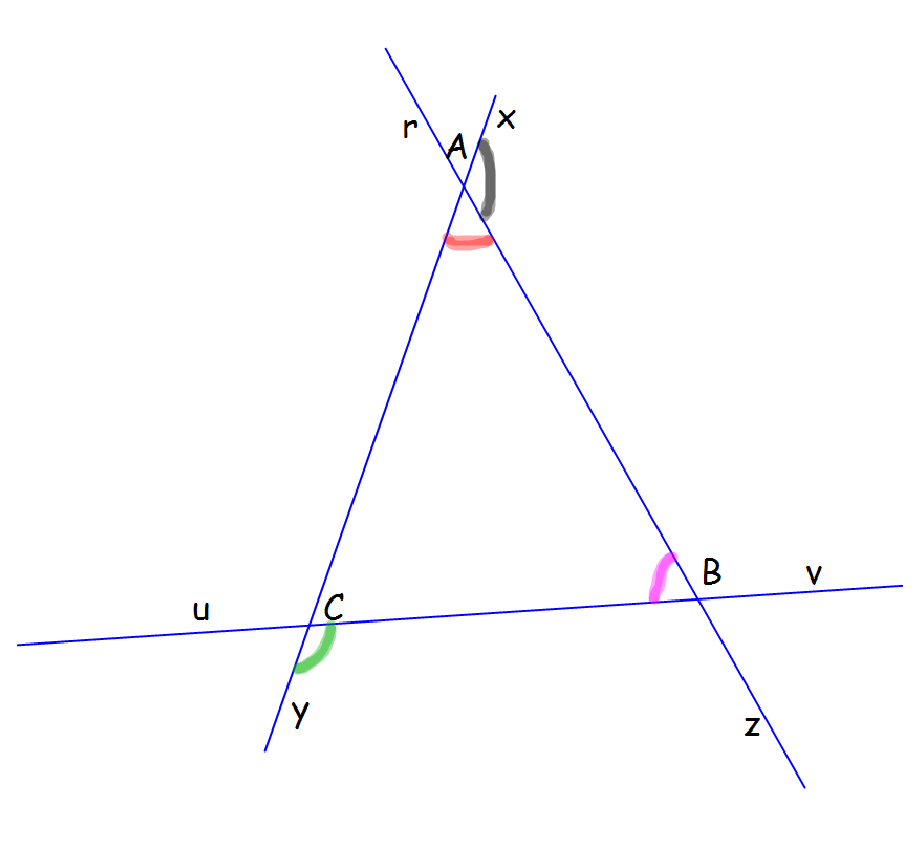
\includegraphics[scale=1]{notationangles1.eps} \\

\initq \q
\initqa \qa L'angle $\widehat{vBA}$ est celui formé par les demi-droites
. . . . .  et . . . . .\\

\qa L'angle $\widehat{uCA}$ est celui formé par les demi-droites . . . . . et . . . . .\\

\q Donner les noms des angles suivants :\\

\initqa \qa rouge : . . . .\\

\qa noir : . . . .\\

\qa rose : . . . .\\

\qa vert : . . . .\\


\vspace*{1cm}


$\rightarrow$ \textbf{Donner la mesure d'un angle à l'aide du rapporteur}\\
\vspace*{0.5cm}


\exo \\ Cliquer sur la mesure des angles représentés ci-dessous (sans utiliser le rapporteur)\\

\begin{tabular}{|c|c|c|c|c|}
\hline 
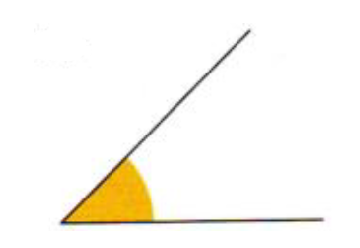
\includegraphics[scale=1]{angle1.eps}  & 15\degre & 45\degre & 65\degre & 145\degre \\ 
\hline 
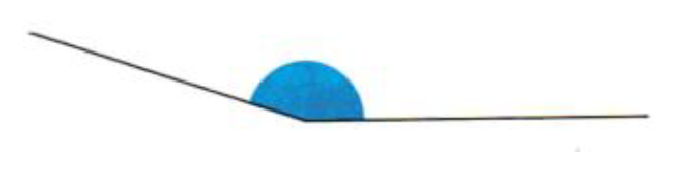
\includegraphics[scale=1]{angle2.eps} & 20\degre & 100\degre & 160\degre & 180\degre \\ 
\hline 
\end{tabular} 


\exo \\ Léo a mal placé son rapporteur pour mesurer l'angle formé des deux demi-droites bleues. Pourquoi ?\\

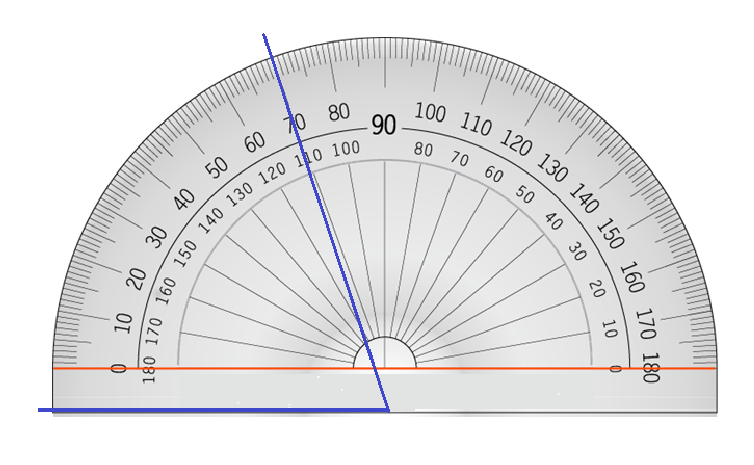
\includegraphics[scale=1]{erreurapporteur.eps} \\

\exo \\ Léa a mal placé son rapporteur pour mesurer l'angle formé des deux demi-droites bleues. Pourquoi ?\\

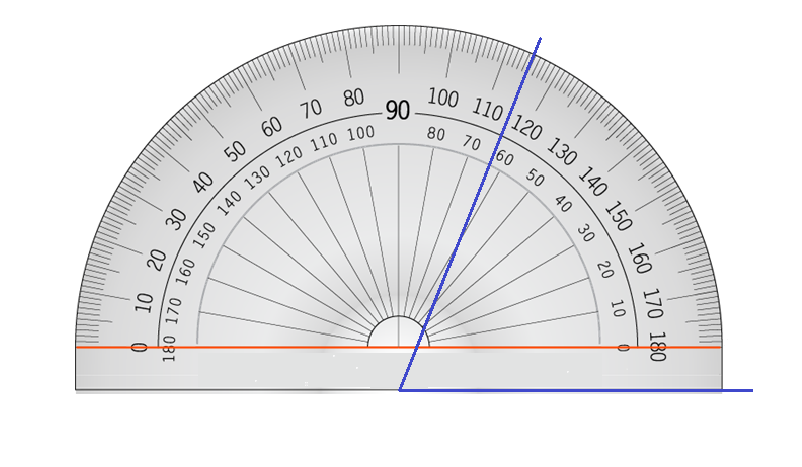
\includegraphics[scale=1]{erreurapporteur2.eps} \\



\exo \\ Mélanie a mesuré 100\degre pour l'angle formé des deux demi-droites bleues. Elle a faux. Pourquoi ?\\


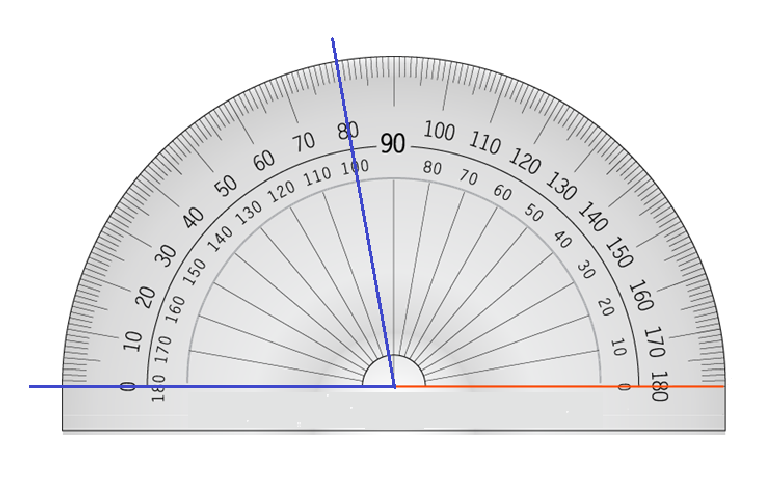
\includegraphics[scale=1]{rapporteur80.eps} \\


\exo \\ Yann a mesuré 70\degre pour l'angle formé des deux demi-droites bleues. Il a faux. Pourquoi ?\\


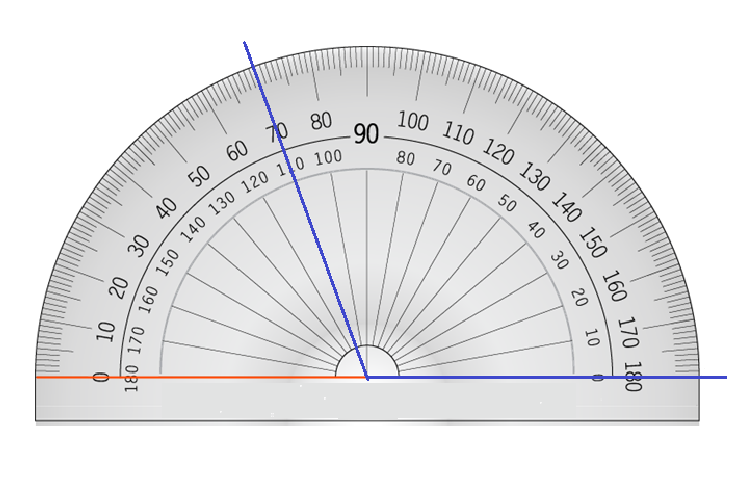
\includegraphics[scale=1]{rapporteur110.eps} \\


\exo \\ Lire à l'aide du rapporteur et écrire la mesure de l'angle formé des deux demi-droites bleues.\\

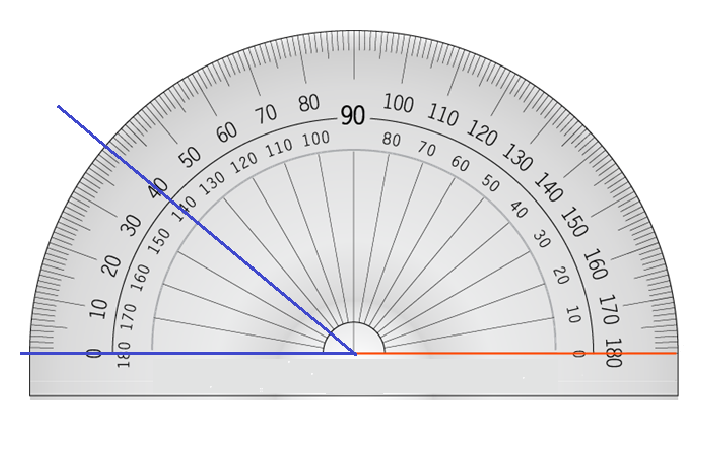
\includegraphics[scale=1]{rapporteur40.eps} \\


\exo \\ Lire à l'aide du rapporteur et écrire la mesure de l'angle formé des deux demi-droites bleues.\\

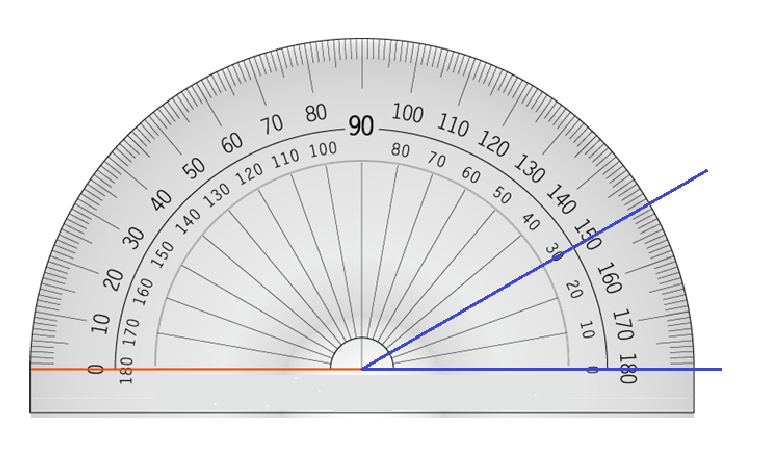
\includegraphics[scale=1]{rapporteur30.eps} \\

\vspace*{0.5cm}

\vspace*{1cm}


$\rightarrow$ \textbf{Exercices de démonstrations}\\
\vspace*{0.5cm}





\exo \\ Dans la figure ci-dessous, les angles $\widehat{xBz}$ et $\widehat{zBy}$ sont adjacents.\\

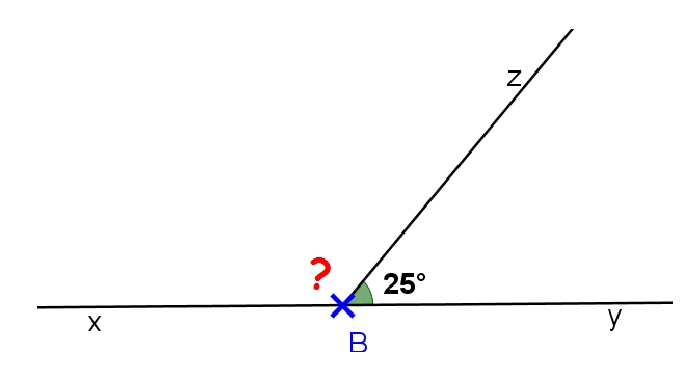
\includegraphics[scale=1]{demo1.eps} \\

Quelle est la mesure de l'angle $\widehat{xBz}$ ?\\

\textbf{Calculs :}\\
\reponse[2]\\


\textbf{Réponse :} L'angle  $\widehat{xBz}$ mesure . . .\degre.\\



\exo \\ Dans la figure ci-dessous, les angles $\widehat{xAz}$ et $\widehat{zAy}$ sont adjacents.\\

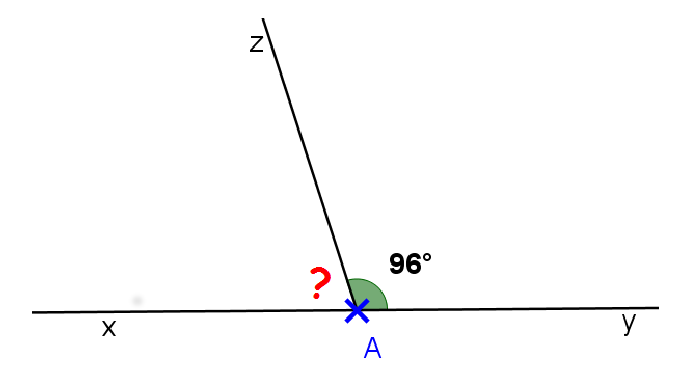
\includegraphics[scale=1]{demo2.eps} \\

Quelle est la mesure de l'angle $\widehat{xAz}$ ?\\

\textbf{Calculs :}\\
\reponse[2]\\


\textbf{Réponse :} L'angle  $\widehat{xAz}$ mesure . . .\degre.\\




\begin{center}
{\Large \textbf{Niveau 2 :}}
\end{center}

\vspace*{1cm}


$\rightarrow$ \textbf{Nommer et reconnaître un angle}\\
\vspace*{0.5cm}


\exo \\ Compléter les définitions des différents types d'angle que l'on peut rencontrer.\\

\initqa \qa Un angle nul est un angle qui mesure . . . degré.\\

\qa Un angle plat, qui mesure . . . degrés.\\


\exo \\ Compléter les définitions des différents types d'angle que l'on peut rencontrer.\\

\initqa \qa Un angle aigu est un angle qui mesure entre . . . . et . . . . degré(s).\\

\qa Un angle droit est un angle qui mesure . . . . degrés.\\

 \qa Un Les angles obtus, qui mesurent entre . . . . et . . . . degrés.\\
 
 
 \exo \\ Compléter le tableau ci-dessous à l'aide de la figure et des mots suivants : \textit{aigu}, \textit{plat}, \textit{droit} et \textit{obtus}.\\
 
 
 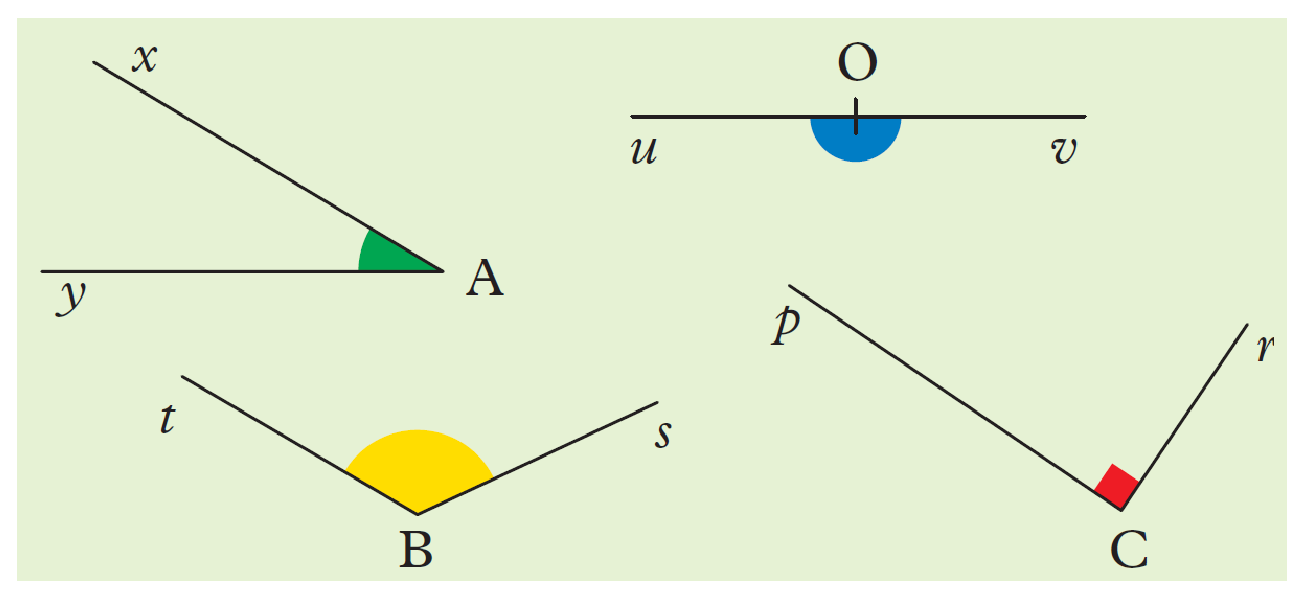
\includegraphics[scale=0.8]{notationangles2.eps} \\
 
 \renewcommand{\arraystretch}{2}
 
\begin{tabular}{|c|c|c|}
\hline 
\textbf{Couleur} & \textbf{Nom de l'angle} & \textbf{Je suis un angle ...} \\ 
\hline 
vert & . . . . & . . . . \\ 
\hline 
jaune & . . . . & . . . . \\ 
\hline 
. . . . & . . . . & droit \\ 
\hline 
. . . . & $\widehat{uOv}$ & . . . . \\ 
\hline 
\end{tabular} 




\exo \\  Classer les angles dans le tableau suivant.\\

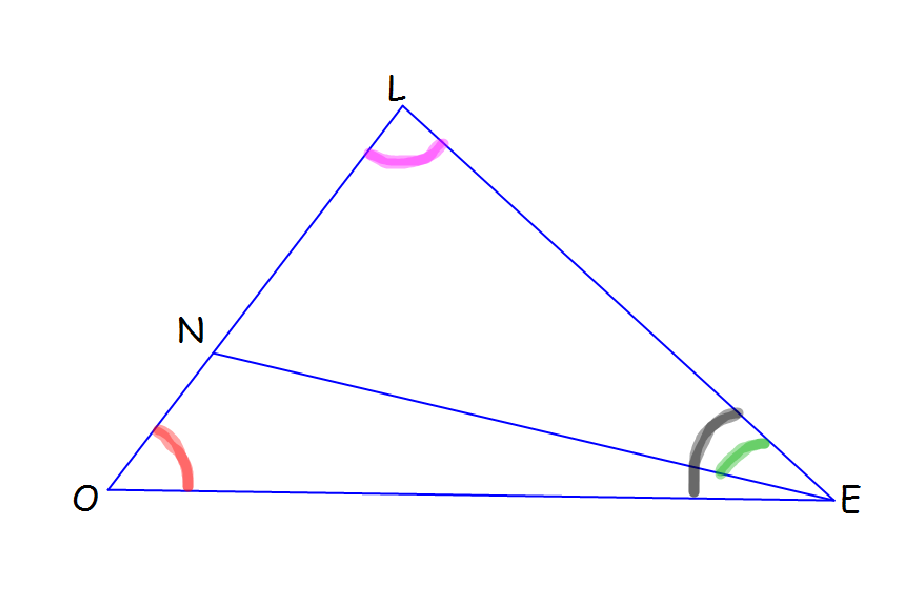
\includegraphics[scale=0.8]{notationangles7.eps} \\

\begin{tabular}{|c|p{10cm}|}
\hline 
Les angles aigus : &  \\ 
\hline 
Les angles obtus : &  \\ 
\hline 
\end{tabular} 

\vspace*{1cm}


$\rightarrow$ \textbf{Donner la mesure d'un angle à l'aide du rapporteur}\\
\vspace*{0.5cm}


\exo \\ Sur les figures ci-dessous, lire et écrire la mesure de chaque angle sur le rapporteur.\\



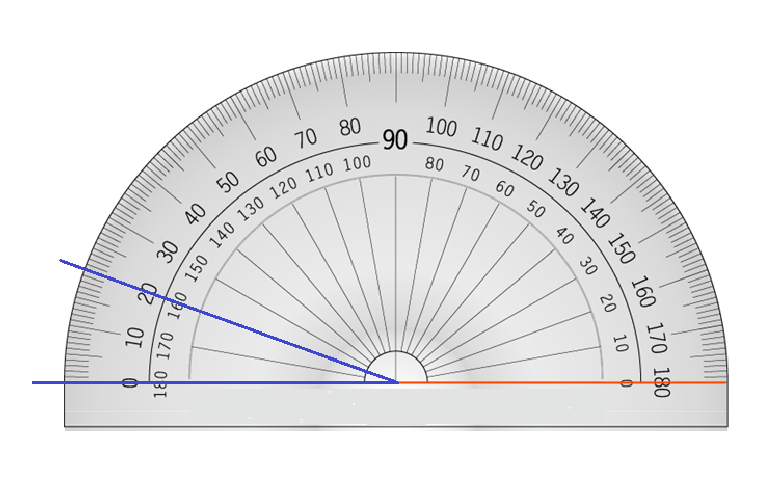
\includegraphics[scale=1]{rapporteur20.eps} \hspace*{1.5cm} . . . .\\


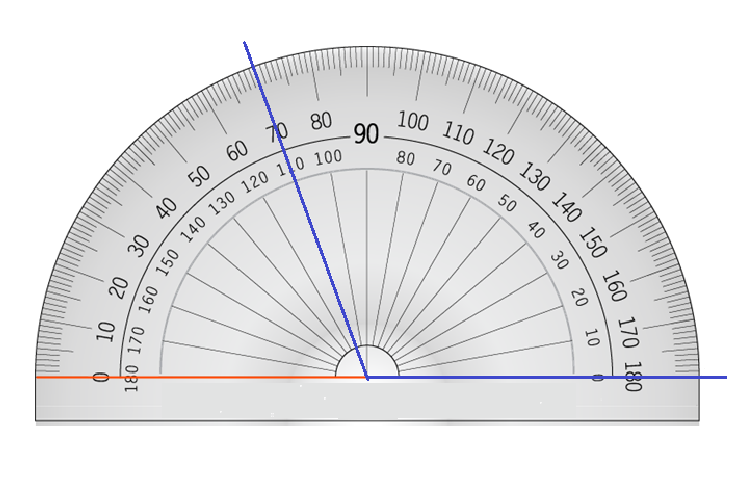
\includegraphics[scale=1]{rapporteur110.eps} \hspace*{1.5cm} . . . .\\




\exo \\ Sur les figures ci-dessous, lire et écrire la mesure de chaque angle sur le rapporteur.\\



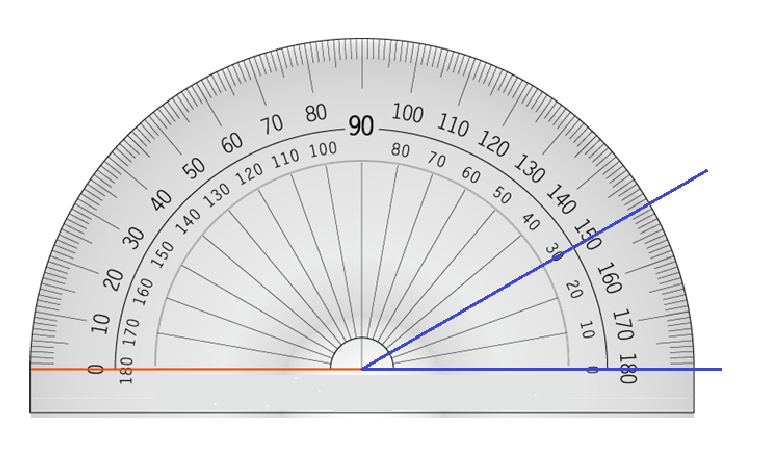
\includegraphics[scale=1]{rapporteur30.eps} \hspace*{1.5cm} . . . .\\



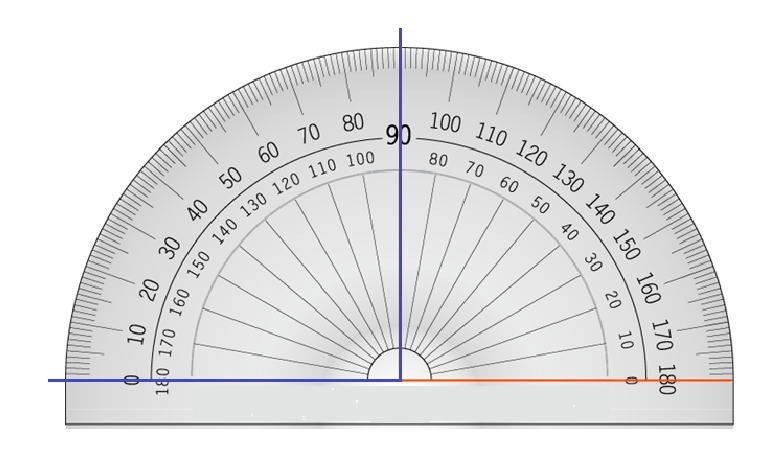
\includegraphics[scale=1]{rapporteur90.eps} \hspace*{1.5cm} . . . .\\



\exo \\ Sur les figures ci-dessous, lire et écrire la mesure de chaque angle sur le rapporteur.\\



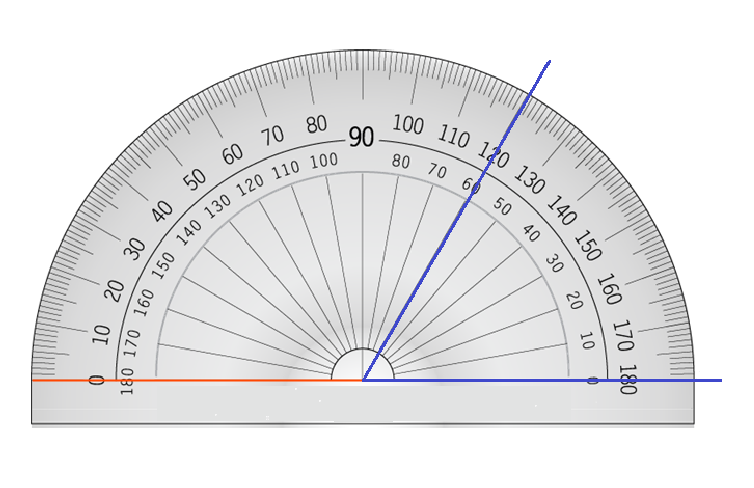
\includegraphics[scale=1]{rapporteur60.eps} \hspace*{1.5cm} . . . .\\


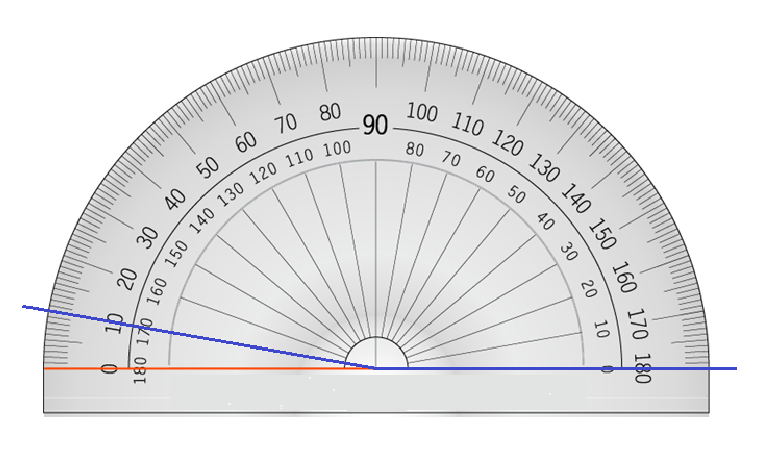
\includegraphics[scale=1]{rapporteur170.eps} \hspace*{1.5cm} . . . .\\

\exo \\ Sur les figures ci-dessous, lire et écrire la mesure de chaque angle sur le rapporteur.\\



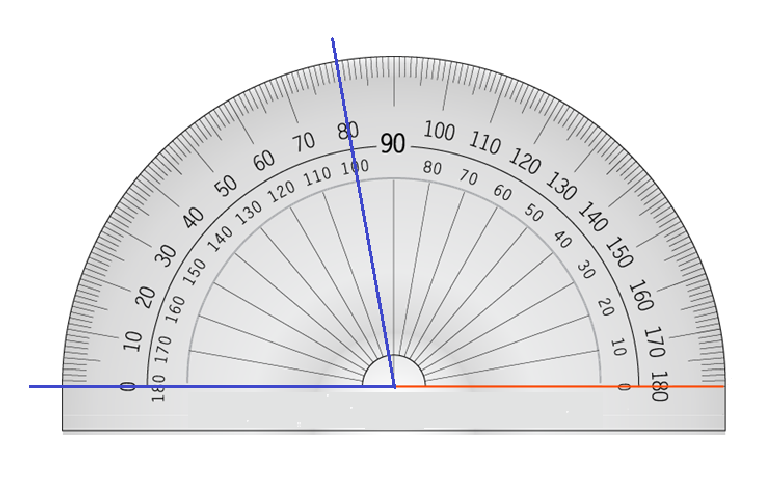
\includegraphics[scale=1]{rapporteur80.eps} \hspace*{1.5cm} . . . .\\


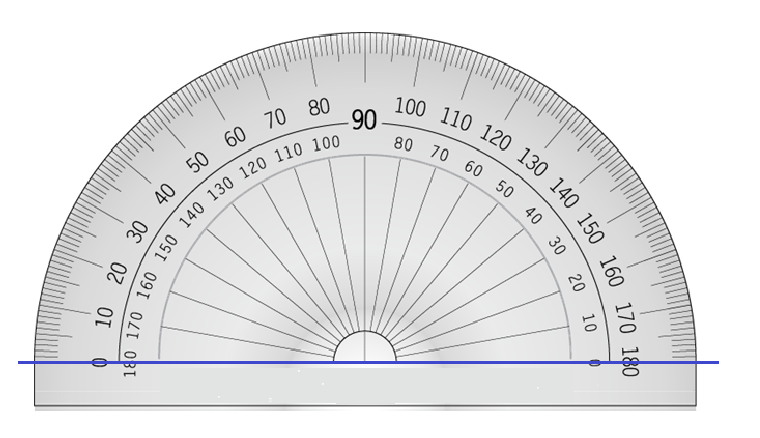
\includegraphics[scale=1]{rapporteur180.eps} \hspace*{1.5cm} . . . .\\

\vspace*{1cm}


$\rightarrow$ \textbf{Exercices de démonstrations}\\
\vspace*{0.5cm}





\exo \\ Dans la figure ci-dessous, les angles $\widehat{qCp}$ et $\widehat{pCn}$ sont adjacents.\\

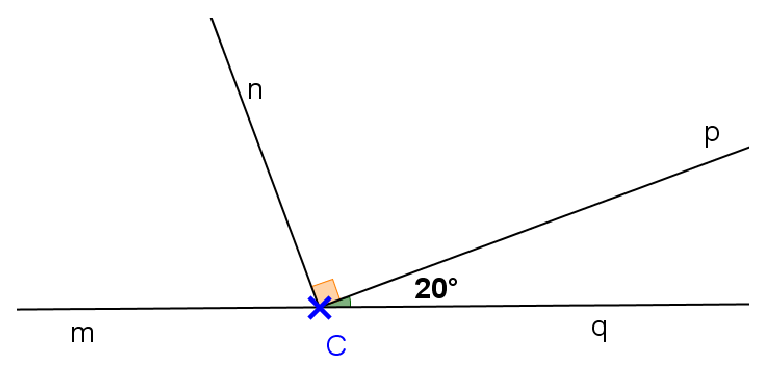
\includegraphics[scale=1]{demo3.eps} \\

Quelle est la mesure de l'angle $\widehat{qCn}$ ?\\

\textbf{Calculs :}\\
\reponse[2]\\


\textbf{Réponse :} \\


\exo \\ Dans la figure ci-dessous, les angles $\widehat{HDG}$ et $\widehat{GDF}$ sont adjacents.\\

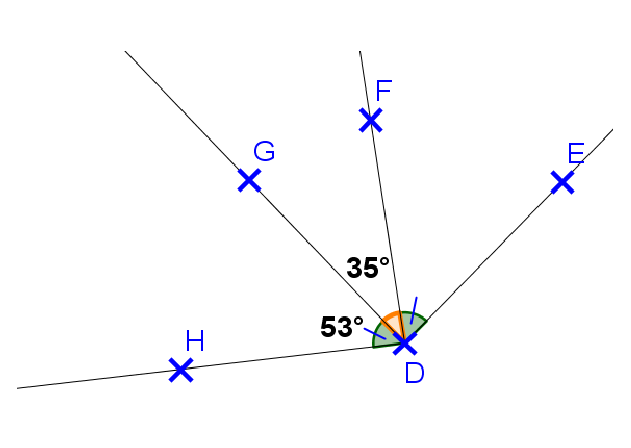
\includegraphics[scale=1]{demo4.eps} \\

Quelle est la mesure de l'angle $\widehat{HDF}$ ?\\

\textbf{Calculs :}\\
\reponse[2]\\


\textbf{Réponse :} \\



\begin{center}
{\Large \textbf{Niveau 3 :}}
\end{center}

\vspace*{1cm}

$\rightarrow$ \textbf{Nommer et reconnaître un angle}\\

\vspace*{0.5cm}


\exo \\ Donner le nom de chacun des angles.\\

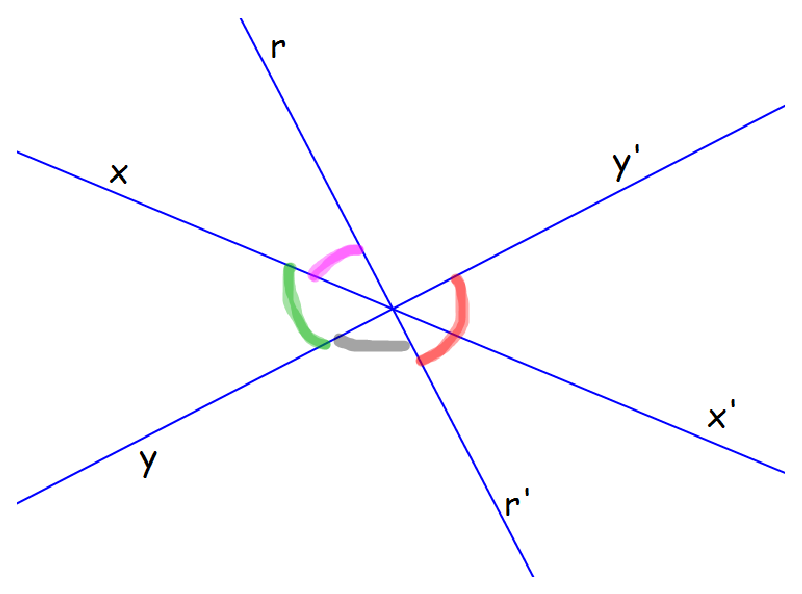
\includegraphics[scale=0.8]{notationangles6.eps} \\

\initqa \qa rose : . . . .\\

\qa rouge : . . . .\\


\qa gris : . . . .\\


\qa vert : . . . .\\

\exo \\ Compléter le tableau ci-dessous.\\

\begin{flushleft}
\begin{tabular}{|p{2cm}|c|c|c|}
\hline 
 &  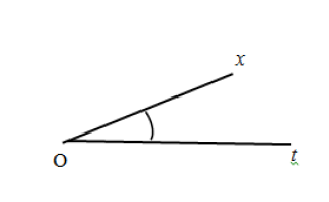
\includegraphics[scale=0.8]{notationangles3.eps} &  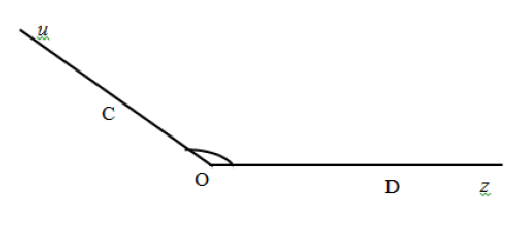
\includegraphics[scale=0.8]{notationangles4.eps} &  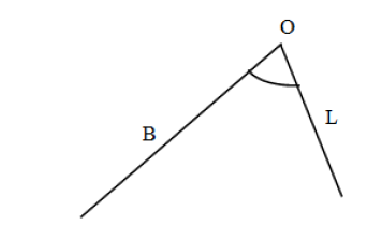
\includegraphics[scale=0.8]{notationangles5.eps} \\ 
\hline 
Nom de l'angle & . . . . & . . . . & . . . . \\ 
\hline 
Je suis un angle ... & . . . . & . . . . & . . . . \\ 
\hline 
\end{tabular} 
\end{flushleft}




\exo \\ Compléter le tableau ci-dessous comme sur l'exemple en observant la figure.\\


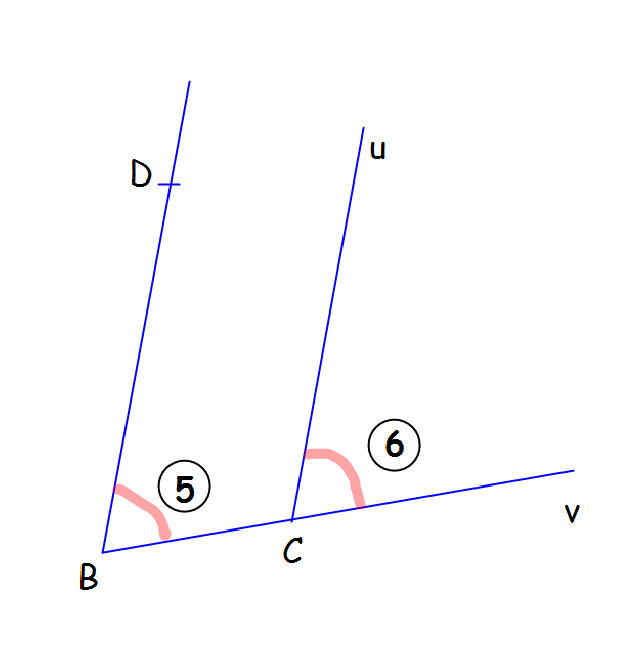
\includegraphics[scale=0.8]{notationangles8.eps} \\

\begin{tabular}{|c|c|c|c|}
\hline 
\textbf{Angle} & \textbf{Notation} & \textbf{Sommet} & \textbf{Côtés} \\
\hline 
EXEMPLE & $\widehat{MLK}$ & L & [LM) et [LK)\\  
\hline 
5 & . . . . & . . . . & . . . . et . . . . \\ 
\hline 
6 & . . . . & . . . . & . . . . et . . . . \\ 
\hline 
\end{tabular} 


\vspace*{1cm}


$\rightarrow$ \textbf{Donner la mesure d'un angle à l'aide du rapporteur}\\
\vspace*{0.5cm}


\exo \\ Sur les figures ci-dessous, lire et écrire la mesure de chaque angle sur le rapporteur.\\



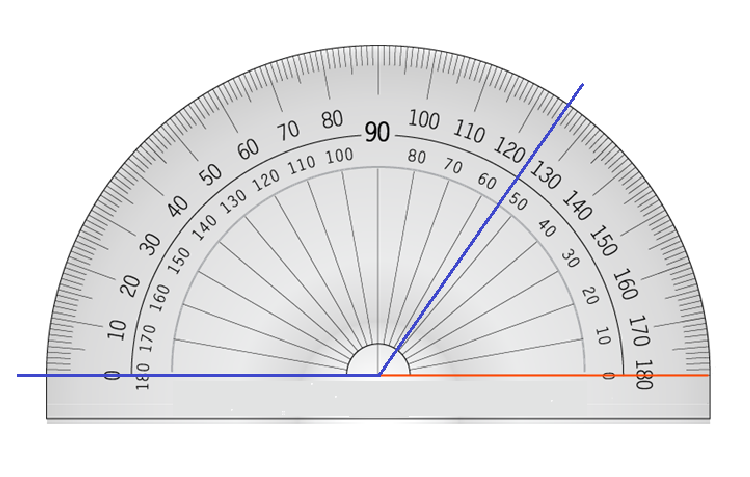
\includegraphics[scale=1]{rapporteur125.eps} \hspace*{1.5cm} . . . .\\



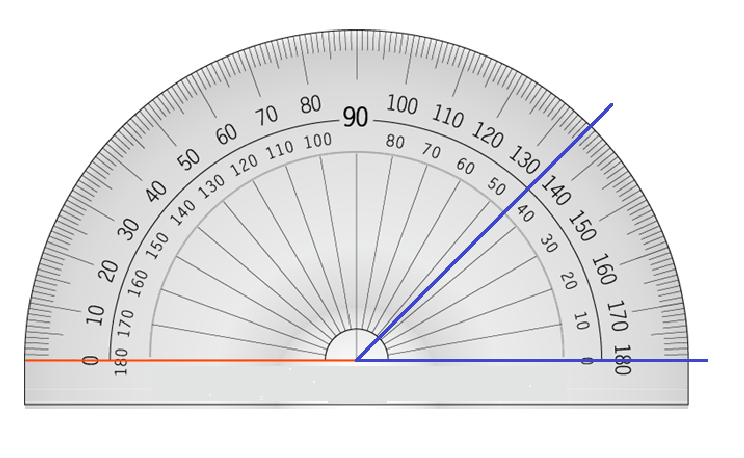
\includegraphics[scale=1]{rapporteur45b.eps} \hspace*{1.5cm} . . . .\\

\exo \\ Sur les figures ci-dessous, lire et écrire la mesure de chaque angle sur le rapporteur.\\



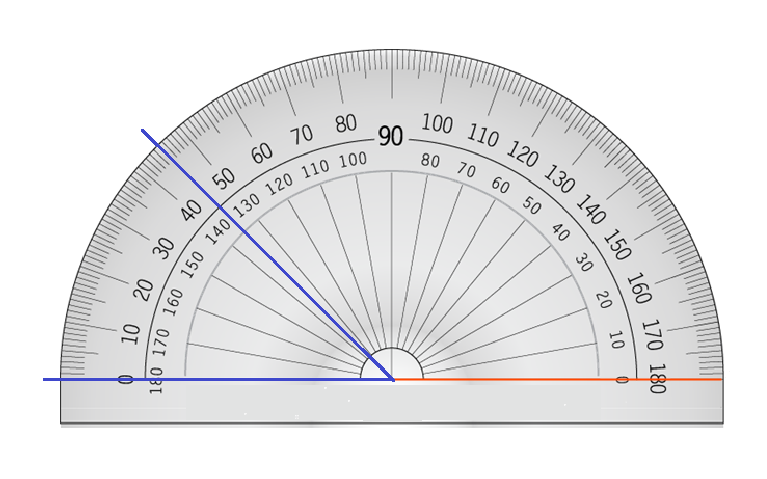
\includegraphics[scale=1]{rapporteur45.eps} \hspace*{1.5cm} . . . .\\



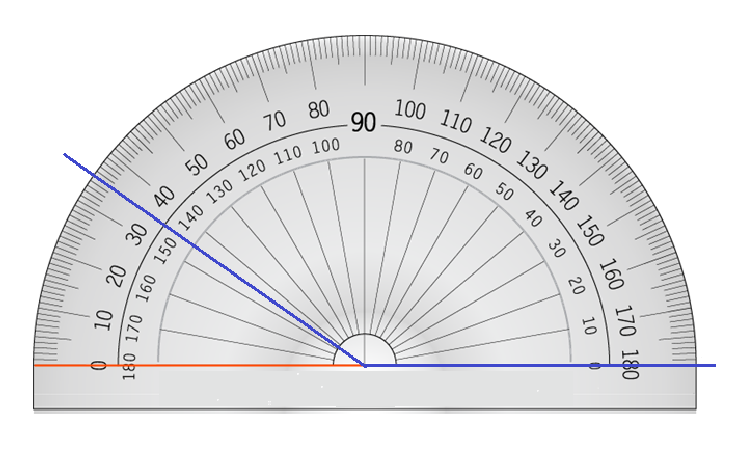
\includegraphics[scale=1]{rapporteur145.eps} \hspace*{1.5cm} . . . .\\



\exo \\ Sur les figures ci-dessous, lire et écrire la mesure de chaque angle sur le rapporteur.\\



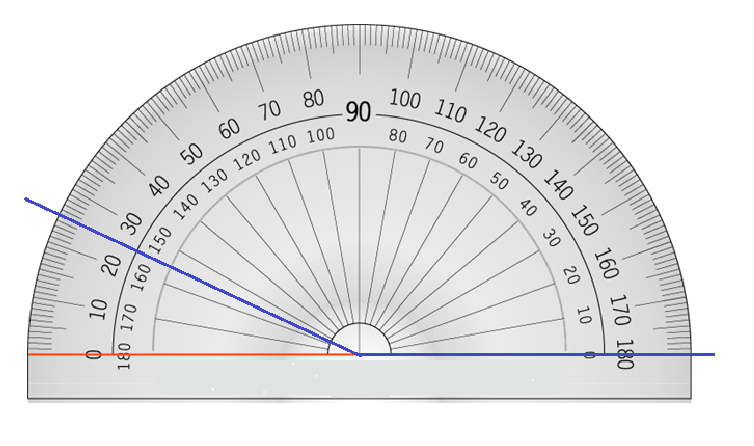
\includegraphics[scale=1]{rapporteur155.eps} \hspace*{1.5cm} . . . .\\



\includegraphics[scale=1]{rapporteur15.eps} \hspace*{1.5cm} . . . .\\






\vspace*{1cm}


$\rightarrow$ \textbf{Exercices de démonstrations}\\
\vspace*{0.5cm}



\exo \\ Dans la figure ci-dessous, les angles $\widehat{qCp}$ et $\widehat{pCn}$ ainsi que $\widehat{pCn}$ et $\widehat{nCm}$ sont respectivement adjacents.\\

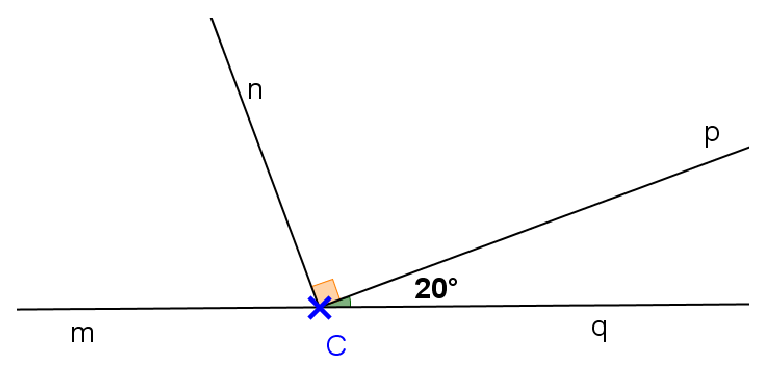
\includegraphics[scale=1]{demo3.eps} \\

Quelle est la mesure de l'angle $\widehat{mCn}$ ?\\

\textbf{Calculs :}\\
\reponse[2]\\


\textbf{Réponse :} \\
\reponse[2]\\





\exo \\ Dans la figure ci-dessous, les angles $\widehat{HDG}$ et $\widehat{GDF}$ ainsi que $\widehat{GFD}$ et $\widehat{FDE}$ sont respectivement adjacents.\\

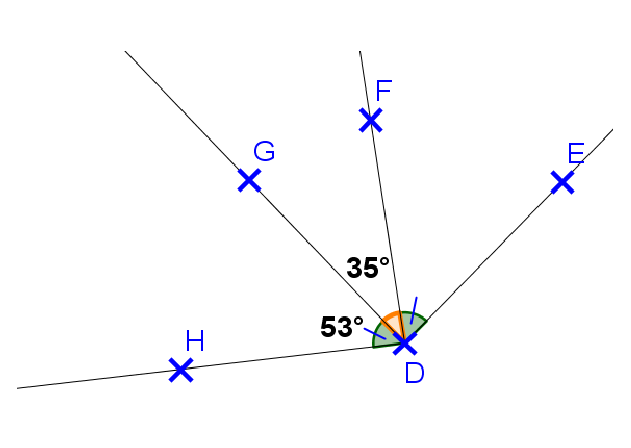
\includegraphics[scale=1]{demo4.eps} \\

Quelle est la mesure de l'angle $\widehat{HDE}$ ?\\

\textbf{Calculs :}\\
\reponse[2]\\


\textbf{Réponse :} \\
\reponse[2]\\


\exo \\ Dans la figure ci-dessous, les angles $\widehat{HDG}$ et $\widehat{GDF}$ ainsi que $\widehat{GFD}$ et $\widehat{FDE}$ sont respectivement adjacents.\\

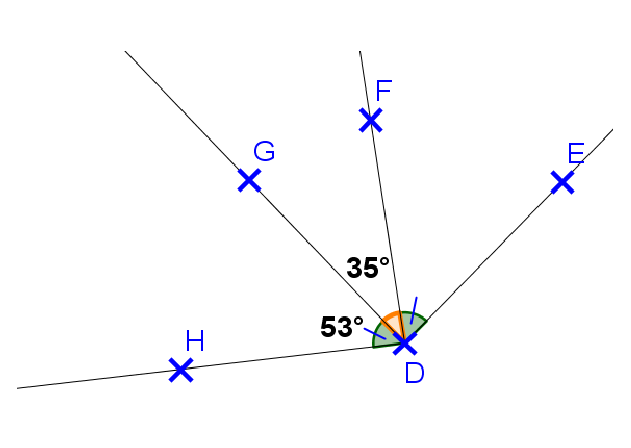
\includegraphics[scale=1]{demo4.eps} \\

Quelle est la mesure de l'angle $\widehat{GDE}$ ?\\

\textbf{Calculs :}\\
\reponse[2]\\


\textbf{Réponse :} \\
\reponse[2]\\




\begin{center}
{\Large \textbf{Niveau 4:}}
\end{center}

\vspace*{1cm}

$\rightarrow$ \textbf{Nommer et reconnaître un angle}\\

\vspace*{0.5cm}


\exo \\ Compléter le tableau ci-dessous comme sur l'exemple en observant la figure.\\


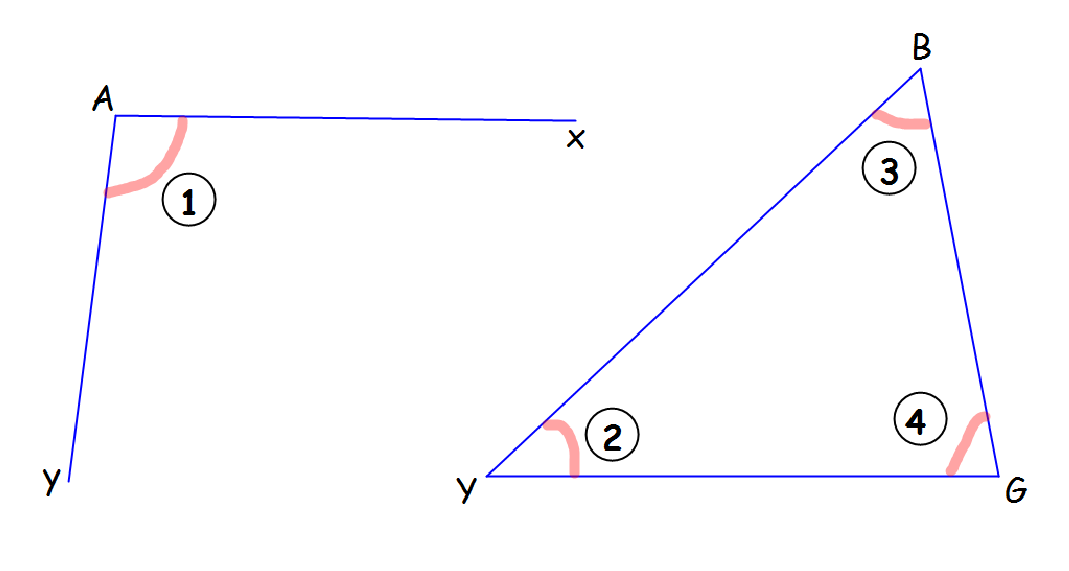
\includegraphics[scale=0.8]{notationangles9.eps} \\

\begin{tabular}{|c|c|c|c|}
\hline 
\textbf{Angle} & \textbf{Notation} & \textbf{Sommet} & \textbf{Côtés} \\
\hline 
EXEMPLE & $\widehat{MLK}$ & L & [LM) et [LK)\\  
\hline 
1 & . . . . & . . . . & . . . . et . . . . \\ 
\hline 
2 & . . . . & . . . . & . . . . et . . . . \\ 
\hline 
3 & . . . . & . . . . & . . . . et . . . .\\
\hline 
4 & . . . . & . . . . & . . . . et . . . .\\
\hline 
\end{tabular} 



\vspace*{1cm}


$\rightarrow$ \textbf{Donner la mesure d'un angle à l'aide du rapporteur}\\
\vspace*{0.5cm}




\exo \\ Sur les figures ci-dessous, lire et écrire la mesure de chaque angle sur le rapporteur.\\



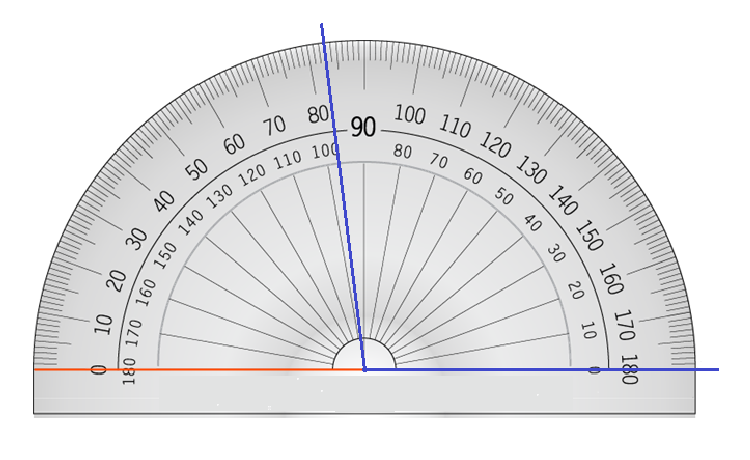
\includegraphics[scale=1]{rapporteur97.eps} \hspace*{1.5cm} . . . .\\



\includegraphics[scale=1]{rapporteur149.eps} \hspace*{1.5cm} . . . .\\





\vspace*{1cm}


$\rightarrow$ \textbf{Exercices de démonstrations}\\
\vspace*{0.5cm}





\exo \\Dans la figure ci-dessous, les angles $\widehat{qCp}$ et $\widehat{pCn}$ ainsi que $\widehat{pCn}$ et $\widehat{nCm}$ sont respectivement adjacents.\\

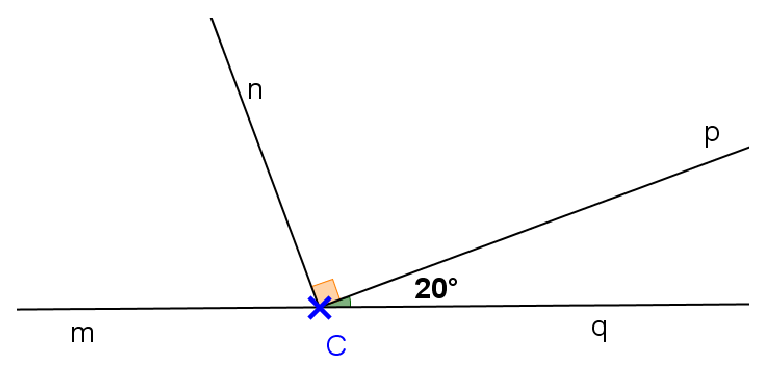
\includegraphics[scale=1]{demo3.eps} \\

Quelle est la mesure de l'angle $\widehat{mCp}$ ?\\

\textbf{Calculs :}\\
\reponse[2]\\


\textbf{Réponse :} \\
\reponse[2]\\


\exo \\ Dans la figure ci-dessous, que représente la droite (xt) pour l'angle $\widehat{zOt}$ ?\\

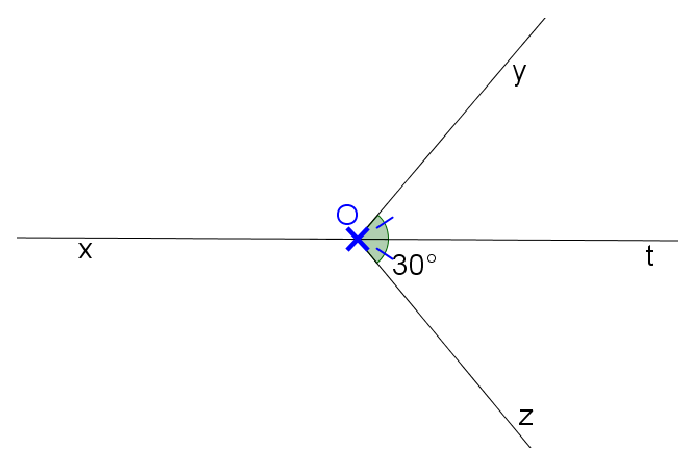
\includegraphics[scale=1]{demo7.eps} \\



\textbf{Réponse :} \\
\reponse[2]\\



\exo \\ Dans la figure ci-dessous, les angles $\widehat{yOt}$ et $\widehat{tOz}$ sont adjacents. La demi-droite [Ot) est la bissectrice de l'angle $\widehat{zOt}$ \\

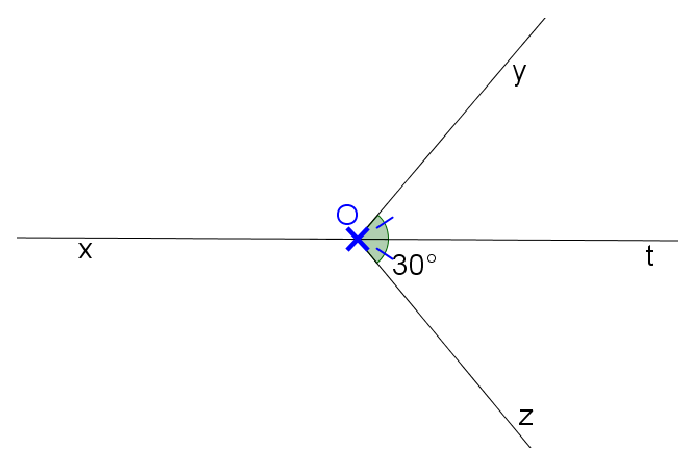
\includegraphics[scale=1]{demo7.eps} \\

Quelle est la mesure de l'angle $\widehat{yOt}$ ?\\

\textbf{Calculs :}\\
\reponse[2]\\

\textbf{Réponse :} \\
\reponse[2]\\


\exo \\ Compléter la définition d'une bissectrice d'un angle.\\

La bissectrice d'un angle est la . . . . . . . . . . . . . . qui partage
un angle en deux angles de même . . . . . . . . . . . .\\








\begin{center}
{\Large \textbf{Niveau 5 :}}
\end{center}

\vspace*{1cm}

$\rightarrow$ \textbf{Nommer et reconnaître un angle}\\

\vspace*{0.5cm}




\exo \\ Compléter le tableau ci-dessous comme sur l'exemple en observant la figure.\\


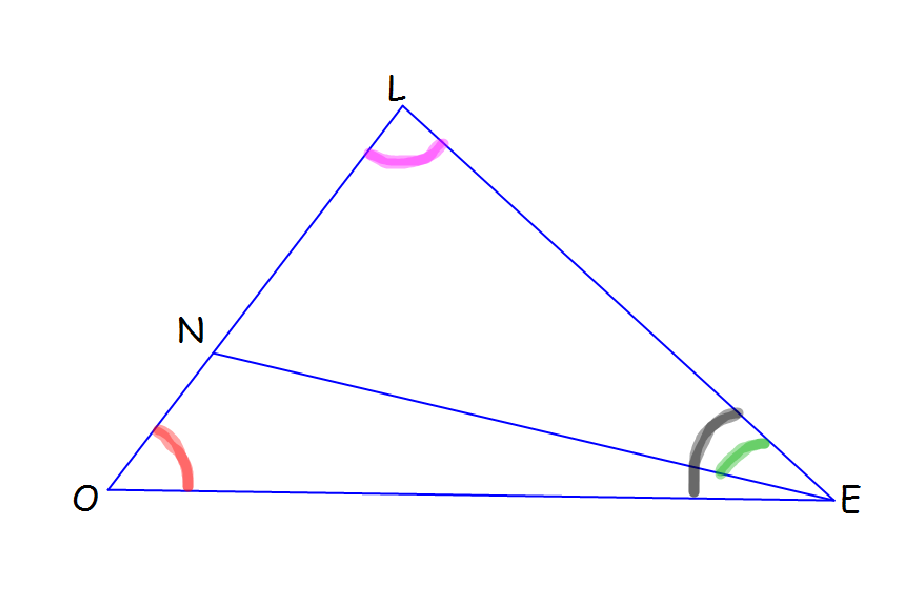
\includegraphics[scale=0.8]{notationangles7.eps} \\

\begin{tabular}{|c|c|c|c|}
\hline 
\textbf{Angle} & \textbf{Notation} & \textbf{Sommet} & \textbf{Côtés} \\
\hline 
EXEMPLE & $\widehat{MLK}$ & L & [LM) et [LK)\\  
\hline 
Vert & . . . . & . . . . & . . . . et . . . . \\ 
\hline 
Noir & . . . . & . . . . & . . . . et . . . . \\ 
\hline 
Rose & . . . . & . . . . & . . . . et . . . .\\
\hline 
Rouge & . . . . & . . . . & . . . . et . . . .\\
\hline 
\end{tabular} 



\vspace*{1cm}


$\rightarrow$ \textbf{Donner la mesure d'un angle à l'aide du rapporteur}\\
\vspace*{0.5cm}





\exo \\ Sur la figure ci-dessous, lire la mesure de chaque angle sur le rapporteur puis compléter les égalités.\\

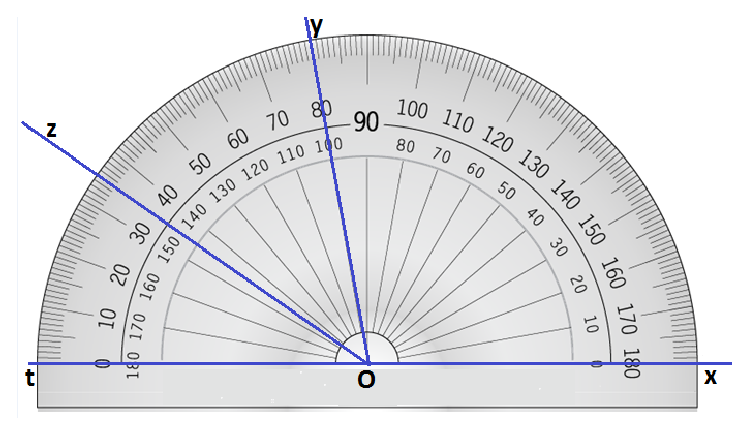
\includegraphics[scale=1]{rapporteurdifficile.eps} \\

\initqa \qa $\widehat{xOy}$ = . . .\\

\qa $\widehat{tOz}$ = . . .\\

\qa $\widehat{xOz}$ = . . .\\

\qa $\widehat{yOt}$ = . . .\\


\exo \\ Sans utiliser le rapporteur, associer chaque angle avec sa mesure parmi la liste suivante : 5\degre, 20\degre, 30\degre, 45\degre, 90\degre, 120\degre, 135\degre, 170\degre.\\

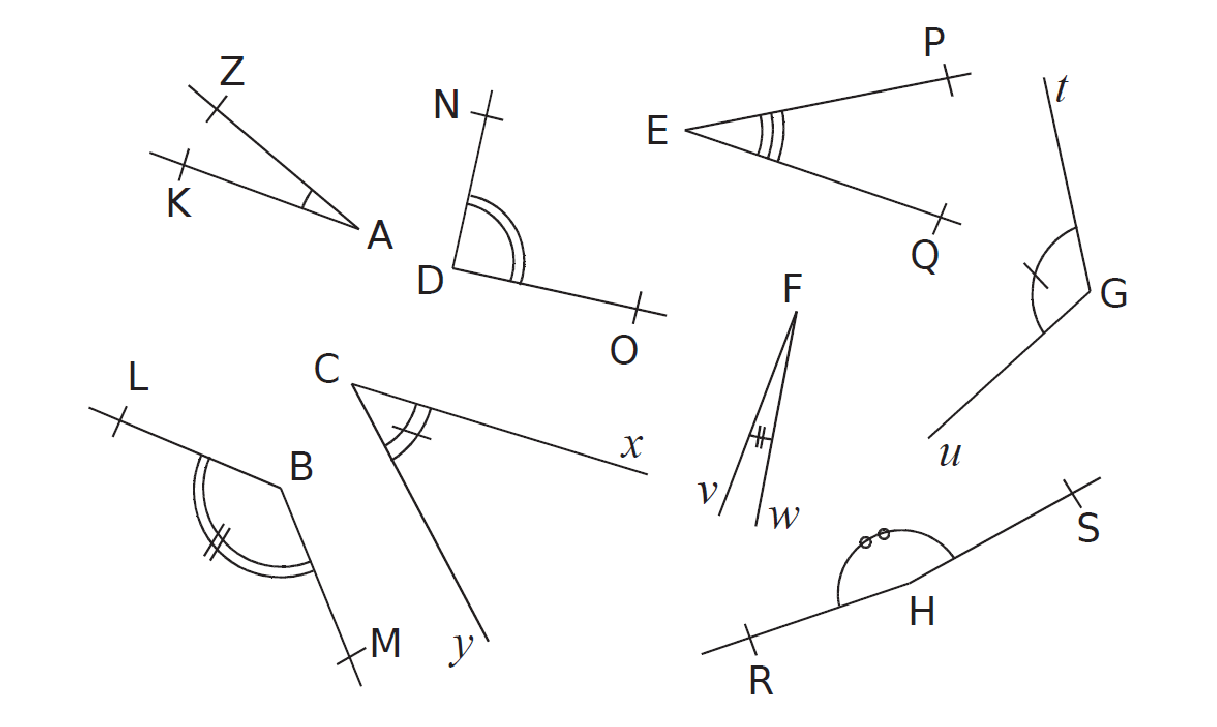
\includegraphics[scale=0.8]{angle3.eps}\\

\initqa 
\qa $\widehat{ZAK}$ = . . . .\\

\qa $\widehat{NDO}$ = . . . .\\

\qa $\widehat{PEQ}$ = . . . .\\

\qa $\widehat{tGu}$ = . . . .\\

\qa $\widehat{LBM}$ = . . . .\\

\qa $\widehat{yCx}$ = . . . .\\

\qa $\widehat{vFw}$ = . . . .\\

\qa $\widehat{RHS}$ = . . . .\\



\vspace*{1cm}


$\rightarrow$ \textbf{Exercices de démonstrations}\\
\vspace*{0.5cm}



\exo \\ Dans la figure ci-dessous, les angles $\widehat{yOt}$ et $\widehat{tOz}$ sont adjacents. La demi-droite [Ot) est la bissectrice de l'angle $\widehat{zOt}$ \\

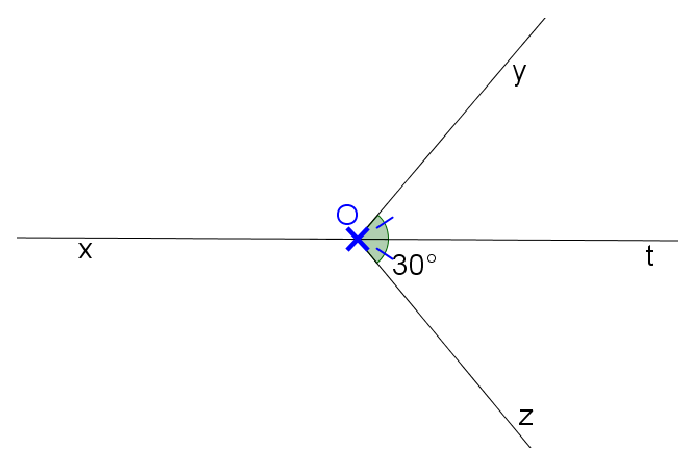
\includegraphics[scale=1]{demo7.eps} \\

Quelle est la mesure de l'angle $\widehat{yOz}$ ?\\

\textbf{Calculs :}\\
\reponse[2]\\

\textbf{Réponse :} \\
\reponse[2]\\

\exo \\ A l'aide de la figure ci-dessous, donner la mesure de  l'angle $\widehat{MDJ}$ ?\\

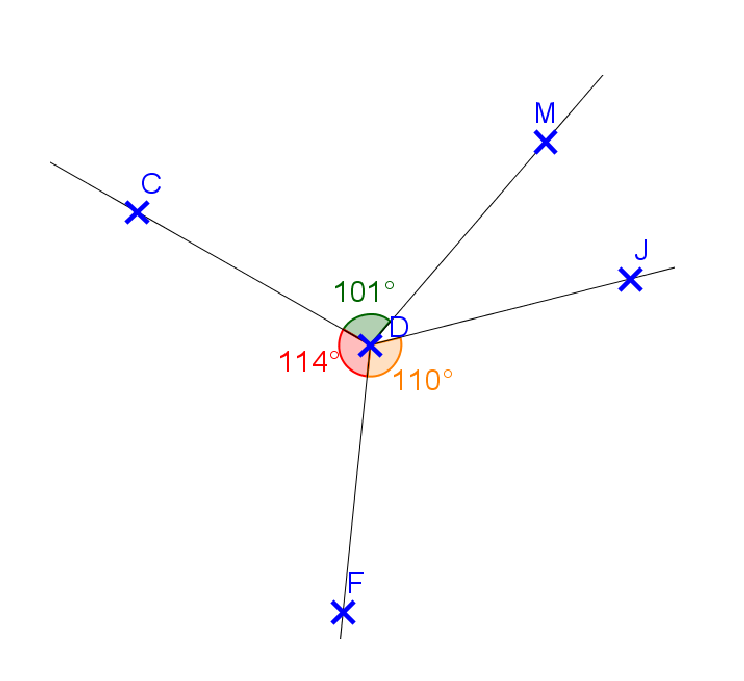
\includegraphics[scale=1]{demo8.eps} \\


\textbf{Calculs :}\\
\reponse[2]\\

\textbf{Réponse :} \\
\reponse[2]\\


\exo \\ En observant la figure ci-dessous, citer une bissectrice.\\

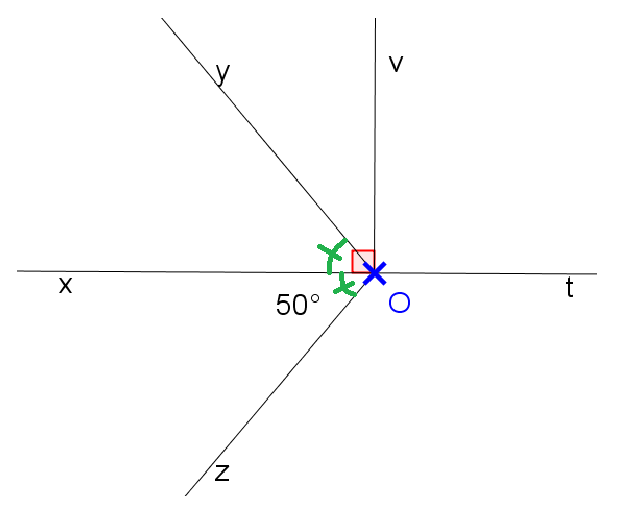
\includegraphics[scale=1]{demo9.eps} \\



\textbf{Réponse :} \\
\reponse[2]\\


\exo \\ Dans la figure ci-dessous, la demi-droite [Ox) est la bissectrice de l'angle $\widehat{yOz}$. \\ 

Quelle est la mesure de l'angle $\widehat{yOv}$?\\

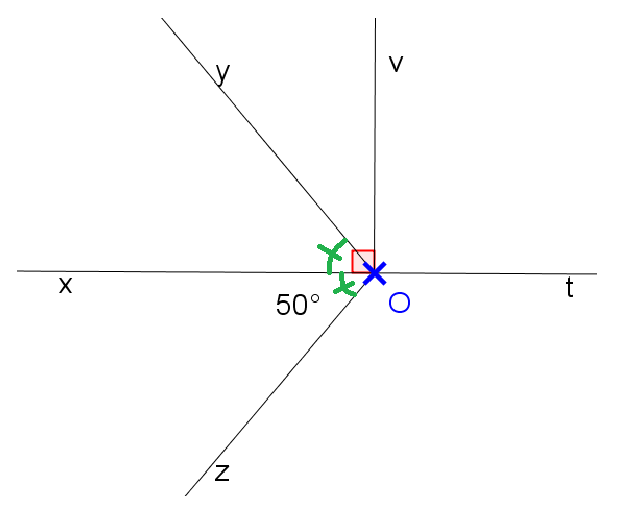
\includegraphics[scale=1]{demo9.eps} \\

\textbf{Calculs :}\\
\reponse[2]\\

\textbf{Réponse :} \\
\reponse[2]\\


\exo \\ Attention, la figure suivante est volontaire fausse. \\

\includegraphics[scale=1]{demo5.eps} \\

Les points A, C et B ci-dessus sont-ils alignés ? Justifier votre réponse.\\

\textbf{Calculs :}\\
\reponse[2]\\


\textbf{Réponse :} \\
\reponse[2]\\



\exo \\ Attention, la figure suivante est volontaire fausse. \\

\includegraphics[scale=1]{demo6.eps} \\

Les points H, S et G ci-dessus sont-ils alignés ? Justifier votre réponse.\\

\textbf{Calculs :}\\
\reponse[2]\\


\textbf{Réponse :} \\
\reponse[2]\\


\end{document}
